\documentclass[a4paper,twoside]{style/article}
\usepackage{epsfig}
\usepackage{subfigure}
\usepackage{calc}
\usepackage{amssymb}
\usepackage{amstext}
\usepackage{amsmath}
\usepackage{amsthm}
\usepackage{multicol}
\usepackage{pslatex}
\usepackage{apalike}
\usepackage{style/SCITEPRESS}
\usepackage[small]{caption}

\subfigtopskip=0pt
\subfigcapskip=0pt
\subfigbottomskip=0pt

% My Packages and Commands ---
\usepackage[normalem]{ulem}
\usepackage{xcolor}
\usepackage[ruled,vlined]{algorithm2e}
\usepackage[utf8]{inputenc}
\usepackage{url}
\newcommand{\rem}[1]{\textcolor{red}{\sout{#1}}}
\newcommand{\add}[1]{\textcolor{blue}{\uline{#1}}}
\newcommand{\com}[1]{\textcolor{orange}{\uline{#1}}}
% /My Packages and Commands --

% modify floating spacings 
% \addtolength{\abovecaptionskip}{-0.0mm}
% \addtolength{\belowcaptionskip}{-0.0mm}
% \addtolength{\dbltextfloatsep}{-5.0mm}
% \addtolength{\textfloatsep}{-4mm}
% \addtolength{\intextsep}{-5.0mm}
%
% % modify paragraph spacings
% \addtolength{\parskip}{-5.0mm}

\begin{document}

\title{Interactive Visual Analysis of Lumbar Back Pain  \subtitle{What the Lumbar Spine Tells About Your Life} }

% \author{Blind}
\author{\authorname{Paul Klemm\sup{1}, Sylvia Glaßer\sup{1}, Kai Lawonn\sup{1}, Marko Rak\sup{1} Henry Völzke\sup{2}, Katrin Hegenscheid\sup{3} and Bernhard Preim\sup{1}}
\affiliation{\sup{1} Department of Simulation and Graphics, University of Magdeburg, Germany}
\affiliation{\sup{2} Institute for Community Medicine, University of Greifswald, Germany}
\affiliation{\sup{3} Institute for Diagnostic Radiology and Neuro-Radiology, University of Greifswald, Germany}
\email{\{klemm, glasser\}@isg.cs.uni-magdeburg.de}
}

\keywords{Epidemiology, Interactive Visual Analysis, Classification, Multi-Modal Data}

\abstract{ 
Epidemiology aims to provide insight into disease causations.
%%
Hence, subject groups (cohorts) are analyzed to correlate the subjects' varying lifestyles, their medical properties and diseases.
%%
Recently, these cohort studies comprise medical image data.
%%
We assess potential relations between image-derived variables of the lumbar spine with lower back pain in a cross-sectional study.
%%
Therefore, an Interactive Visual Analysis (IVA) framework was created and tested with 2,540 segmented lumbar spine data sets.
%%
The segmentation results are evaluated and quantified by employing shape-describing variables, such as the spine canal course, its curvature and torsion.
%%
We analyze mutual dependencies among shape-describing variables and non-image variables, e.g. pain indicators.
%%
Therefore, we automatically extract a decision tree classifier for each non-image variable.
%%
We provide an IVA technique to compare classifiers with interactive scatter plot visualizations.
%%
As a first result, we conclude that image-based variables are only sufficient for classification of lifestyle factors within the data.
%%
A correlation between lumbar spine shape and lower back pain was not existent in the automatically trained classifiers.
%%
However, the presented approach is a valuable extension for the IVA of epidemiological data.
%%
Hence, relations between non-image variables were successfully detected and characterized.
}

\onecolumn \maketitle \normalsize \vfill

\section{\uppercase{Introduction}}
\label{sec:Introduction}

\noindent Epidemiology is the study of dissemination, causes and results of health-related states and events.
%%
For this purpose, large population studies, such as the \emph{Study of Health in Pomerania} (SHIP) \cite{SHIP}, gather as much information as possible about participants to be assessed towards different diseases.
%%
This information is used to determine risk factors for diseases, help people to live healthier or to support the diagnosis of widespread diseases.
%%
% So far, epidemiological research is strongly hypothesis-driven.
% %%
% More precisely, observations made by clinicians are translated into hypotheses, which are then statistically evaluated using data variables from epidemiological studies.
% %%
% As a result, the hypothesis will be accepted or rejected.
% %%
%%
Cohort studies are an instrument of epidemiological research.
%%
Nowadays, these studies often comprise medical image data, e.g., tomographic image data sets. %, as well as general patient-specific attributes, such as \emph{gender}, \emph{age} and \emph{weight}.
%%
We analyze back pain, one of the most frequent complaints in the Western civilization. %\cite{Hoy2010}. % and gains importance due to the population aging \cite{Hoy2010}.
%%
Epidemiological analysis of back pain aims to determine risk factors.
%%
Although the shape and constitution of the spine, especially the lumbar spine, plays an important role for back pain, an automatic classification approach for characterization of back pain based on lumbar back spine attributes is still missing.
%%
%Furthermore, previous analyses mainly focused on a single variable (e.g. \emph{BMI}) or a small subset of variables.
%%

We present an analysis of the image-derived data from a cohort study lumbar spine dataset.
%%
We extract possible associations between spine shape and back pain characteristics.
%%
For this purpose, we combine data mining algorithms with data visualization techniques.
%%
Then, Interactive Visual Analysis (IVA) highlights mutual dependencies between image-derived data and back pain-related variables.
%%
% The workflow is part of an IVA framework, constructed to enhance the epidemiological workflow with iterative data-driven techniques.
%%
We focus on highlighting new correlations and trigger \emph{hypotheses generation}, rather than statistically validate complex epidemiological correlations.
%%
Our contributions are:
\begin{itemize}
\item An IVA workflow for back pain analysis based on image-derived variables of 2,240 subjects,
%%
\item The identification of lumbar spine shape properties potentially associated with back pain,
%%
\item The detection of associations between image-based, socio-demographic and medical variables for hypothesis generation,
%%
\item The identification of the most important variables via data mining methods using a novel semi- quantitative overview visualization concept. % embedded in our IVA-framework.
%%
\end{itemize}
%%
%The analysis, as well as the presented IVA tool is available as supplementary material in an interactive \texttt{R Markdown}\footnote{Developed by RStudio, Inc; \texttt{rmarkdown.rstudio.com}} document (\url{blind.dnsalias.com}).
%%
%% ---------------------------------------------
\section{\uppercase{Epidemiological Background}}
\label{sec:EpidemiologicalBackground}
%%
\noindent Epidemiological reasoning relies on a strict statistically-driven workflow \cite{Fletcher}:
%%
\begin{itemize}
%%
	\item Physicians formulate hypotheses based on observations made in their clinical practice.
%%
	\item Epidemiologists compile a list of variables depicting a hypothesis to prove it.
%%
	\item Statistical methods, such as regression analysis, assess the correlation of selected variables with the investigated disease.
%%
\end{itemize}
%%
Mutually dependent variables make this analysis challenging.
%%
Many diseases, such as different cancer types, are more likely with increasing age \cite{Fletcher}.
%%
% For example, the effect of nutrition on prostate cancer requires age normalization due to the increased incidence for older subjects.
% %%
% Age acts as a \emph{risk factor} for prostate cancer.
% %%
% Statistical correlation does not imply causation--epidemiologists need to assess the medical soundness of the statistical results.
%%------------------------------
\paragraph{Challenges of Epidemiological Data Analysis.}
% Epidemiological data originates from a wide range of studies.
% %%
% The study type depends on the condition of interest.
% %%
% Most common are case-control studies analyzing one specific disease and its influence on the human body.
%%
We focus on epidemiological large scale cohort study data.
%%
These studies aim at collecting as much data as possible for each subject.
%%
The collected data can be analyzed regarding many diseases and conditions.
%%
Epidemiological data are heterogenous and incomplete.
%%
For example, data about a disease treatment only affects subjects suffering from this condition.
%%
Therefore, statistical analysis has to take missing data into account.
%%
Epidemiological data acquisition includes a variety of techniques, such as medical examinations, self-reported questionnaires or genetic examinations.
%%
This yields a heterogenous information space.
%%
Information reduction techniques are necessary to compare these data.
%%
For example, continuous data, such as age, is often discretized into quantile bins for visualizing age-dependent disease frequencies.

Modern cohort studies often comprise medical image data.
%%
The analysis of these data is challenging.
%%
Individual diagnosis or manual segmentation of each body structure by radiologists is tedious, costly and comprises little reproducibility.
%%
Segmentation algorithms are not generally available and need to be carefully adapted for each body structure.
%%
%Segmentation data is usually analyzed by abstracting it into key figures, such as diameters or distances.
%%
%These numeric values can be compared with non-image variables to retrieve correlations.
%%--------------------------------
\\\\
\noindent \textbf{Lower Back Pain.}
%%
Lower back pain is one of the most frequent complaints in the Western civilization \cite{Hoy2010}.
%%
% Epidemiologists assume correlations between lumbar back pain and lifestyle factors.
% %%
% These include \emph{nutrition}, \emph{physical activity} and \emph{body posture combined with physical stress at work}.
%%
The exact causes as well as particularly vulnerable risk groups are unknown.
%%
Epidemiologists want to characterize the relation between the aging and degenerative process of the spine \cite{Szpalski2005}.
%%
They have to analyze the lumbar spine shape as well as lifestyle factors.
%% -------------------------------
\section{\uppercase{Related Work}}
\label{sec:RelatedWork}
%%
\noindent \textbf{Visual Analysis of Medical Image and Non-Image Data}
%%
In a previous work, we proposed an extension to the previously described epidemiological workflow using IVA \cite{Klemm2014VIS}.
%%
The workflow consists of an iterative sequence of \emph{group selection}, \emph{variable selection} and \emph{visualization}.
%%
It aims to trigger \emph{hypothesis generation} by providing visualizations able to concurrently analyze multiple heterogenous variables at once using correlation measures.
%%
%We incorporate the IVA approach by concurrently displaying complex relationships between variables via decision trees.
%%
\cite{Steenwijk} propose a coordinated linked view system for both image-related and non-image data.
%%
It incorporates multiple plot types, such as scatter plots, parallel coordinates and time plots with brushing and linking facilities.
%%
Similar to our work, they quantify image data and project it into the non-image data information space.
%%
\cite{Turkay} follow a similar approach by deriving descriptive data metrics from image data.
%%
Their proposed \emph{deviation plot} shows distribution-specific measures of a variable, such as skewness or inter-quantile range, making variables comparable.
%%
This approach aims to trigger \emph{hypothesis generation} by outlining tendencies between these variables.
%%
A survey on image-centric cohort studies and strategies to analyze the resulting data is given in \cite{Preim2014}.
%%
\\\\
\noindent \textbf{Visual Analysis of Heterogenous Non-Image Data.}
%%
\cite{Zhang} analyze subject groups in a web-based linked view system.
%%
The resulting decision rules aim to categorize new subjects as they are added to the data.
%%
They define a cohort as variable-divided subject group, differing from the epidemiological understanding of the term.
%%
The described method lacks details about handling of missing data, the definition of similarity or the choice of the statistical measures.
%%
Generalized Pairs Plots (\texttt{GPLOM'S}) visualize heterogenous variables in a plot matrix \cite{GPLOMS,Francois}.
%%
The plot depends on the type of variables, which are visualized pairwise.
%%
\texttt{GPLOM'S} are well suited for an overview visualization, but take up much screen space and are therefore only suitable for few variables at once (see example in Fig.~\ref{fig:image-parameter-range} later on).
%%
% \cite{Dai} define a \emph{Concept Map}, linking cancer-associated features by incorporating choropleth maps with bar charts, parallel coordinates and scatter plots with regression lines.
% %%
% The \emph{Concept Map} is iteratively refined using primarily the underlying geographical data.
%%
%%----------------------------
\\\\
\noindent \textbf{Decision Rule-Driven Analysis of Medical Data.}
Related work in this field often focuses on clinical diagnosis.
%%
Closest to ours is the work of \cite{Glasser2013} and \cite{Niemann2014}.
%%
Both use decision trees for their analyses.
%%
Decision trees are easily readable and are well suited for classifying medical data.
%%
The effort of analyzing decision trees increases with their complexity.
%%
\cite{Glasser2013} use variables derived from DCE-MRI data capturing the perfusion in tumorous tissue.
%%
To classify breast tumors, they train a decision-tree classifier, concluding that the extracted kinetic and morphological features alone are not sufficient for tumor type classification.
%%
\cite{Niemann2014} assess hepatic steatosis (fatty liver disease) risk factors using decision trees.
%%
They present an interactive data mining tool, which can analyze association rules and highlight interesting relations, which may trigger new hypotheses about the data.
%%
We combine both ideas by validating the significance of image-derived variables.
We aim at deriving new relationships by training decision trees to explain target variables.
%%----------------------------
%%
\cite{Pinheiro} applied association rule mining to create high-confidence decision rules based on variables, such as age, gender and geographic location about the mortality rate in liver cancer data.
%%
% \cite{Sekhavat} propose an interactive visualization technique for decision trees, where all decisions are displayed in a heat map.
% %%
% The visualization translates the decision tree into a heat map, where each cell represents the connectivity between an initial and a target value.
% %%
% The resulting interactive visualization is well suited for analyzing single, but not multiple decision trees.
%%
\\\\
\noindent \textbf{SHIP Data Analysis.}
\cite{Klemm2013VMV} analyzed the lumbar spine variability of 490 \texttt{SHIP-2} subjects.
%%
They incorporate hierarchical agglomerative clustering to derive shape groups, yielding several groups of average shape and several outlier clusters.
%%
The extracted lumbar spine shape was correlated with subject size.
%%
Our data extraction process is based on the detection algorithm and lumbar spine canal extraction presented by \cite{Klemm2013VMV}.
%%
Clustering techniques are strongly dependent on the chosen variables and distance measures \cite{Klemm2014BVM}.
%%
\\\\
Unique in our work is the combination of data mining techniques with an IVA approach by observing interesting feature relations in the context of image-derived features using multiple decision trees for one visualization.
%%
We abstract the decision tree results similar to \cite{Turkay}, making them comparable in an overview visualization.
%%
\section{\uppercase{The Lumbar Spine Data Set}}
\label{sec:MaterialsAndMethod}
%%
% \noindent Our approach allows the simultaneous analysis of many variables.
%%
%Therefore, epidemiologists compiled the data set with a wide range of variables possibly correlating with lumbar back pain.
\noindent Epidemiologists compiled a data set with a wide range of variables possibly correlating with lumbar back pain, comprising non-image and image-derived data for 6,753 subjects
%%
%The data set comprises 6,753 subjects from two cohorts (4,420 from \texttt{SHIP-Trend-0} and 2,333 from \texttt{SHIP-2}) including non-image and image-derived data.
%%
\\\\
\noindent \textbf{Non-Image Data}.
%%
The non-image variables range from somatometric variables describing body measures to medical examinations, such as laboratory tests as well as lifestyle factors, e.g. sporting activity or nutrition.
%%
The data set comprises 134 variables: %(and 9 additional image-derived variables described in the next subsection):
\begin{itemize}
	\item 21 metric variables, describing somatometric variables and markers retrieved from blood analysis
	%%
	\item 113 categorical variables divided into
	%%
	\begin{itemize}
		%%
		\item 43 dichotomous (binary) variables, mostly indicating the presence of a disease, e.g. \emph{pancreatitis} or \emph{high blood pressure}
		%%
		\item 70 variables with more than two levels, indicating pain levels, nutrition and social factors, such as marital or retirement status
		%%
	\end{itemize}
%%
\end{itemize}
%%
% Many variables comprise missing data.
% %%
% Some variables are follow-up questions, covering the treatment of a disease.
% %%
% Others are exclusive to subgroups, such as women-specific variables, e.g. \emph{menstrual status}.
% %%
% Sparse variables are statistically less resilient and need to be treated with care during the analysis.
\noindent \textbf{Image-Derived Data.}
\begin{figure}[!t]
  %\vspace{-0.2cm}
  \centering
  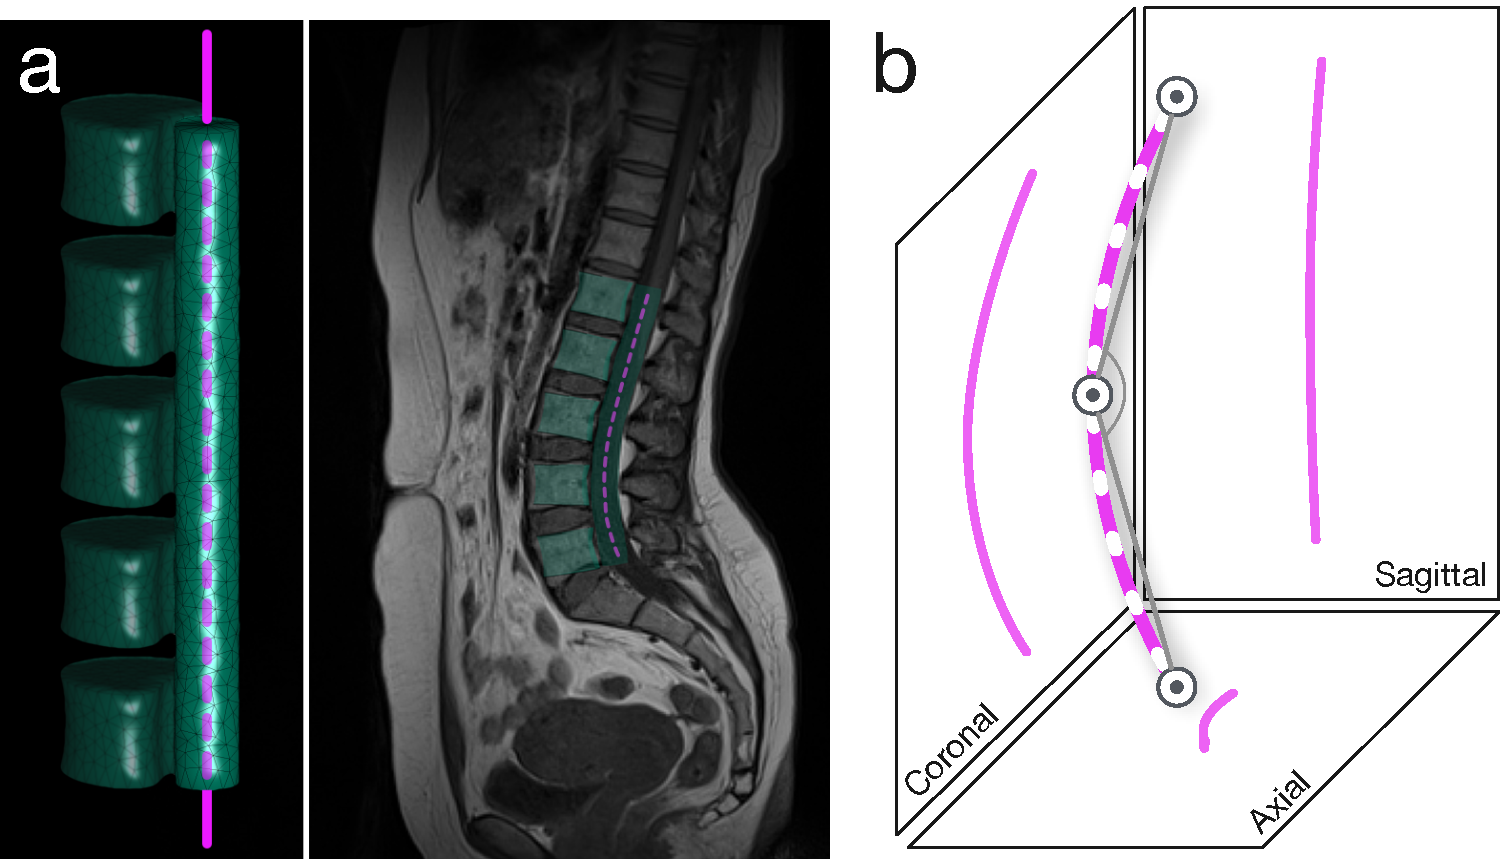
\includegraphics[width=0.475\textwidth]{figures/centerline}
  \caption{
	(a) Finite element model (FEM) of the lumbar spine (left), capturing the L1-L5 vertebrae and the lumbar spine canal (right).
	%%
%	(a) right: FEM aligned to an MRI data set.
	%%
	%The purple dashed line represents the centerline, describing the lumbar spine canal with 92 points.
	The purple dashed line describes the lumbar spine canal centerline with 92 points.
	%%
	(b) We extract the weighted sum of \emph{curvature} and \emph{torsion} for all 92 points (white dashes).
	%%
	The \emph{curvature angle} ($\alpha$) is calculated using the top, bottom and middle point.
	%%
	We extracted the variables for each projection axis to assess their information gain.
	}
  \label{fig:centerline}
\end{figure}
Magnetic Resonance Imaging (MRI) scans were obtained for each subject \cite{Hegenscheid2013}.
%%
% Four trained radiologists acquired the medical image data for each subject in a standardized way using a 1.5~Tesla Magnetic Resonance Imaging (MRI) scanner (Magnetom Avanto; Siemens Medical Solutions, Erlangen, Germany).
% %%
% The spine protocol consisted of a sagittal $T_1$- and $T_2$-weighted turbo-spin-echo sequence ($1.1\times1.1\times4.0~mm$ voxels) \cite{Hegenscheid2013}.
% %%
%%
A hierarchical finite element method was used to detect the lumbar spine in the MRI data \cite{Rak2013}.
%%
%The tetrahedron-based finite element model (Fig.~\ref{fig:centerline}~a) is initialized using three user-defined landmarks.
%%
%A click on the L3 vertebra center initializes the model, two clicks on the top and bottom of the vertebra describe an initial height estimation (Fig.~\ref{fig:centerline}~a).
%%
The tetrahedron-based finite element model (Fig.~\ref{fig:centerline}~a) captures information about the lumbar spine canal shape and the position of the L1-L5 vertebrae.
%The registered model captures information about the lumbar spine canal shape and the position of the L1-L5 vertebrae.
%%
%Each subject's model is mapped to a common reference frame using procrustes analysis to compensate for differences in translation, rotation and scaling.
%%
The detection fails for several subjects due imaging artifacts or strongly deformed spines, yielding models for $2,540$ out of $6,753$ subjects.
%%
%$2,540$ out of $6,753$ lumbar spine models were obtained and constitute the foundation of this work.
%%
%We have to assess the model accuracy to extract key figures from it.
%%
The detection model depicts the vertebrae positions, spine canal curvature, but lacks detailed information about their volume.
%%
%It captures reliable information about spine canal curvature.
%%
In \cite{Klemm2013VMV}, we extracted a centerline representation of the lumbar spine canal from the detection model (Fig.~\ref{fig:centerline}~a).

%%
Using the Frenet frame, we calculated the following metrics from the model (Fig.~\ref{fig:centerline}~b): %\cite{Frenet}:
%%
\begin{itemize}
	\item \emph{Mean Curvature} is calculated as weighted sum of curvature between all adjacent points describing the centerline: $\sum_{i=1}^I \frac{curvature_i}{I}$. We refer to total curvature as \emph{curvature}.
%%
	\item \emph{Mean Torsion} (deviation of a curve from its current course) is calculated as weighted sum of torsion between all adjacent points describing the centerline: $\sum_{i=1}^I \frac{torsion_i}{I}$. We refer to total torsion as \emph{torsion}.
%%
	\item \emph{Curvature angle $\alpha$} is defined by the middle point of the spine canal centerline as \emph{vertex} and the line between middle point and top/bottom point as \emph{sides}.
%%
\end{itemize}
%%
% These metrics are also extracted in the sagittal, coronal and transversal projection of the model.
% %%
% We assess the information gain of each dimension using these projections.
% %%
% This yields a total of 9 image-derived variables.
These metrics are also extracted in the sagittal, coronal and transversal projection of the model, yielding 9 image-derived variables.
%%
In the next section, we present the experiments we conducted to assess the influence of the lumbar spine shape to lower back pain.
%%
\section{\uppercase{Experiments and Preliminary Results}}
\label{sec:Experiments}
% \begin{figure}[!h]
%   %\vspace{-0.2cm}
%   \centering
%   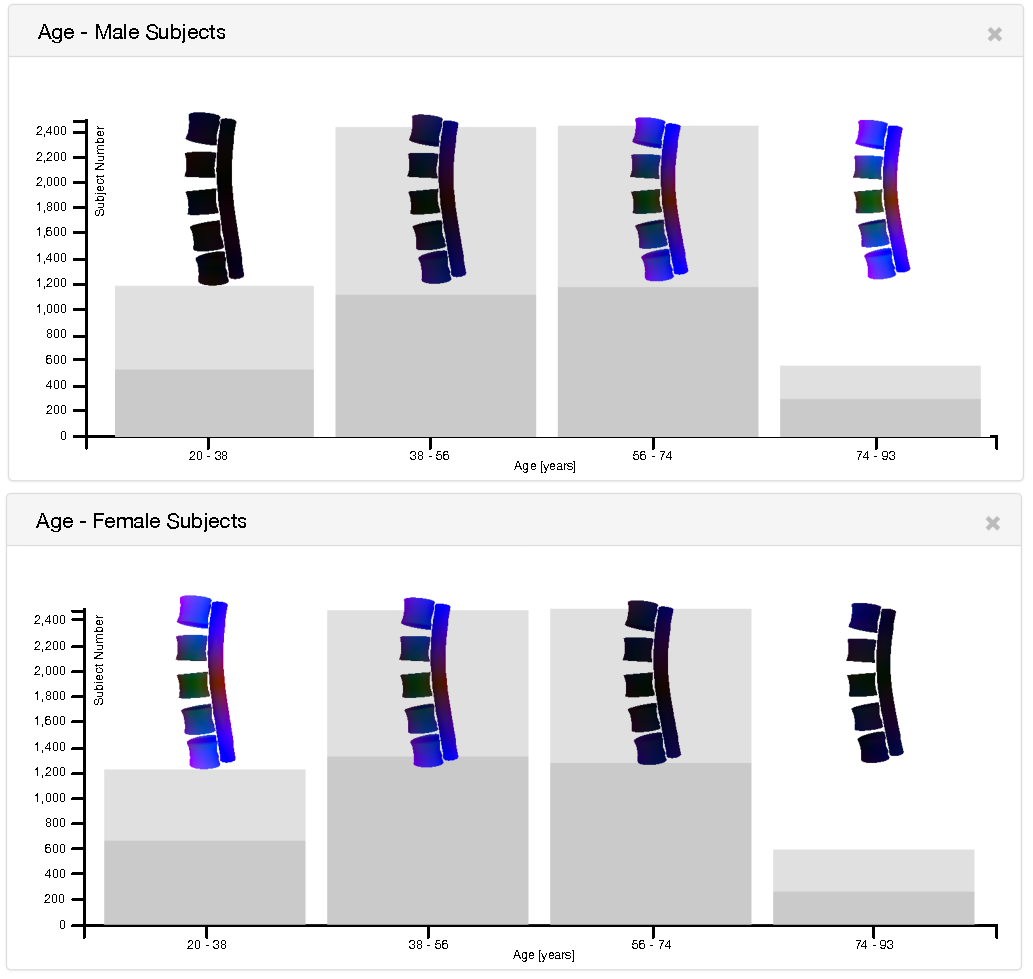
\includegraphics[width=0.475\textwidth]{figures/age-gender}
%   \caption{
% 	%%
% 	Correlation of \emph{age} and \emph{gender} regarding the lumbar spine size.
% 	%%
% 	The bar chart shows subjects divided into four different \emph{age} groups (x-axis) and their subject count (y-axis).
% 	%%
% 	Each bar contains the mean lumbar spine of the respective group.
% 	%%
% 	The shape color encodes the distance (red for x axis, blue for y axis, green for z axis) to the overall male (top chart) or female (bottom chart) mean shape.
% 	%%
% 	The dark gray share of each bar encodes the portion of male (top chart) or female (bottom chart) subjects.
% 	%%
% %	Women have a higher live expectance than men, hence their higher share in the old age group.
% 	%%
% %	Also, women are on average smaller than men, hence the larger shape similarity with older subjects.
% 	%%
% 	%Due to bone erosion, older people are also smaller on average.
% 	}
%   \label{fig:age-gender}
% \end{figure}
%%
\noindent Spine shape is possibly associated with several somatometric variables.
%%
Larger people have also a longer spine with a straighter shape.
%%
Since men are on average taller than women and people of old age shrink due to \emph{bone erosion}, \emph{gender} and \emph{age} are also risk factors.
%%
Women have a higher life expectancy than men, hence their higher share in the old age group.
%%
Also, women are on average smaller than men, hence the larger shape similarity with older subjects.
%%
Large \emph{body weight} increases the spine load, resulting in a bent shape.
%%
To assess their influence, we take them into account when spine \emph{curvature} and \emph{torsion} is correlated with non-image variables.
%%
Since the \emph{gender} encodes \emph{body size}, we decided to divide subjects into \emph{body size} groups.
%%
Discretizing metric variables using quartiles avoids small outlier groups.
%%
\\\\
\noindent \textbf{GPLOM Analysis.}
As a first experiment we correlated the shape variable with the dichotomous back pain indicator using \texttt{GPLOM's} \cite{GPLOMS}.
%%
Since our image-derived variables are metric, their pairwise combinations are visualized using scatter plots.
%%
The combination of the image variables with back pain is visualized as histogram at the left side of the matrix and as box plot on the right side.
%%
Figure~\ref{fig:image-parameter-range} (right) shows the range of each variable as box plot.
%%
The projections to the transversal planes attract attention as they have many outliers.
%%
We conclude that \emph{curvature} is not as reliable on the transversal plane as it is on the other planes.
%%--------------------------------
\\\\
\noindent \textbf{Correlation Matrix.}
\begin{figure*}[htb]
  %\vspace{-0.2cm}
  \centering
  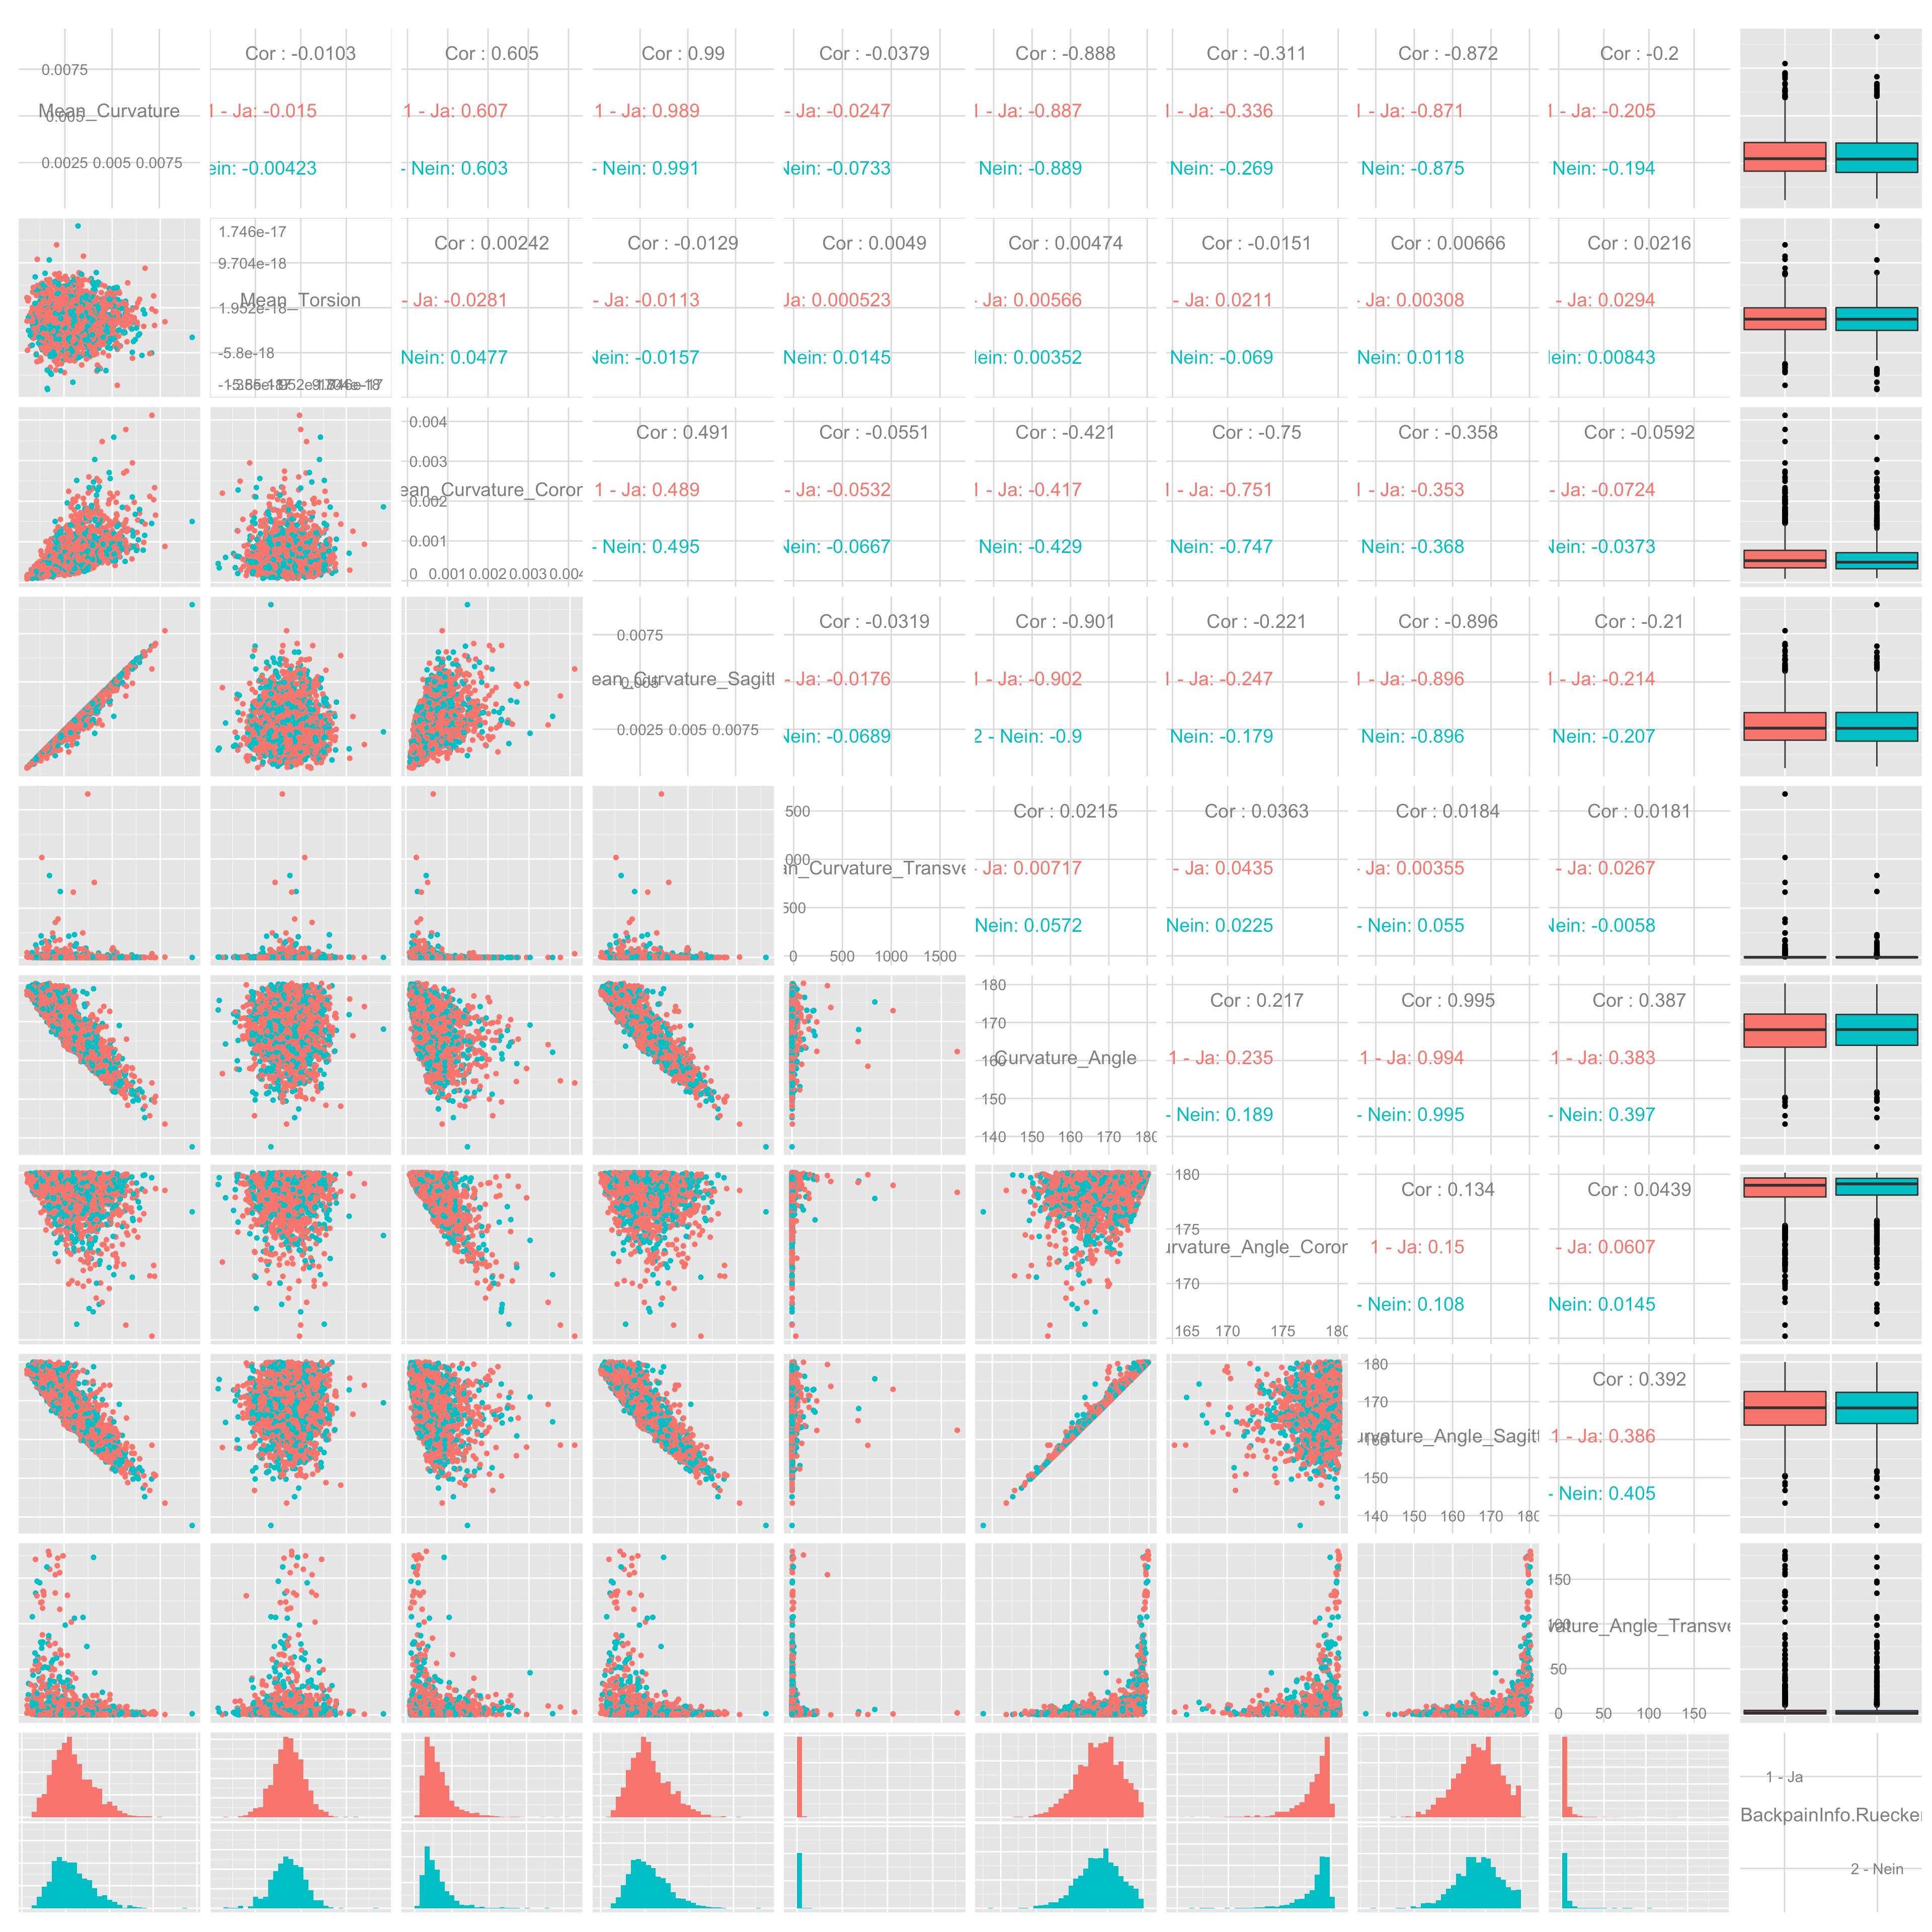
\includegraphics[width=1.0\textwidth]{figures/image-parameter-range}
  \caption{
%%
A Generalized Pairs Plot of all image-derived variables colored by presence (red) or absence (turquoise) of back pain.
%%
Pairwise combinations of image-derived variables are visualized via scatter plots on the left of the matrix diagonal.
%%
Their correlation with back pain is denoted to the right of the matrix diagonal.
%%
The box plots (right) and histograms (bottom) display the distribution of each image variable encoded with back pain.
%%
No correlations with back pain are present as it can be seen in this plot.
}
  \label{fig:image-parameter-range}
\end{figure*}
We calculated a correlation matrix to assess correlations between the image variables.
%%
The pearson correlation coefficients between the numeric variables are depicted right of the matrix diagonal (Fig.~\ref{fig:image-parameter-range}).
%%
\emph{Curvature}, \emph{curvature angle} and \emph{torsion} strongly correlate with their planar projections.
%%
Also the \emph{mean curvature} and \emph{curvature angle} correlate by a factor of $-0.89$.
%%
\emph{Torsion} does not correlate with any other image-derived variable.
%%--------------------------------------------------------
\\\\
\noindent \textbf{Correlation of Image Variables With Lumbar Back Pain.}
Figure~\ref{fig:image-parameter-range} shows the distribution of all image-variables as Generalized Pairs Plot.
%%
No statistically significant correlation could be observed through all subject groups.
%%
The box plots show no difference between subjects with or without back pain.
\\\\
\noindent \textbf{Assessing the Information Gain Using the Principal Component Analysis.}
%%
To determine the information gain per image-derived variable, we calculated a Principal Component Analysis (PCA) and compared the dimension loadings.
%%
The PCA results in a linear projection of the variable space ordering their components by maximum variance.
%%
The first three principal components explain 75\% of the variance in the nine image-derived variables.
%%
The first principal component explains 47\% of the variance and comprises primarily \emph{mean curvature}, \emph{sagittal curvature}, \emph{curvature angle} and \emph{sagittal curvature angle}.
%%
The second component, adding 16\% of the variance, weigths \emph{coronal curvature} and \emph{coronal curvature angle}.
%%
The third component explains 12\% of the variance and comprises \emph{torsion} and \emph{transverse curvature}.
%%
This supports our prior conclusion about the low information gain of the transverse planes.
%%
\emph{Torsion} also adds little variance to the information space.
%%
The complete analysis can be found in the experiments section of the supplementary material (\url{blind.dnsalias.com})
%% ------------------------------------------
\\\\
\noindent \textbf{Heterogenous Correlations.}
%%
We then expanded our focus on correlations of image-derived variables with all other non-image variables.
%%
Different correlation metrics depending on the type of the individual variables are used to derive correlations between all variables in the data set.
%%
The method uses the following correlation metrics for the different type combinations:
%%
\begin{itemize}
%%
\item \emph{Pearson product-moment} for two continuous variables, 
\item \emph{Polyserial} correlation for one continuous and one categorical variable, and
\item \emph{Polychoric} correlations for two categorical variables.
\end{itemize}
%%
All correlation values are scaled between \texttt{0 - no correlation} and \texttt{1 - perfect correlation}.
%%
Some variables are too sparse for calculating correlations, for example \emph{treatment of diabetes}, or \emph{medication against high blood pressure}.
%%
These variables have to be omitted in the analysis, since they are not statistically resilient.
%%
We display the resulting \emph{contingency matrix} using a heat map, encoding correlation values with color brightness with white for $0$ and dark blue for $1$, as presented in \cite{Klemm2014VIS}.
%%
We calculated the contingency matrix for all size groups and searched for correlations between image- and non-image derived variables.
%%
The resulting contingency matrices are available as supplementary material and show no strong correlation with any of the variable (see \url{blind.dnsalias.com}).
%%
Only weak correlations could be found for \emph{mean curvature} with \emph{gender} (0.42), \emph{body size} (0.39) and \emph{number of born children} (0.29).
%%
One surprising result was the small correlation of \emph{torsion} with \emph{Parkinson's disease} (0.24).
%%
Other than that, \emph{torsion} correlated with almost no variables (values between 0 and 0.05).
%%

These observations brought us to the decision to incorporate sophisticated data mining techniques to assess the influence of the image-derived variables.
%%
\section{\uppercase{Evaluation of Decision Trees}}
\label{sec:DecisionTrees}
%%
\noindent As described before, correlation coefficients fail to infer back pain status based on lumbar spine canal \emph{curvature} and \emph{torsion}.
%%
We rely on predictive classification trained to obtain a complex rule set on how combinations of the image-variable explain non-image variables.
%%
Decision trees are a established classification method in data mining to create predictive models.
%%
Leafs of a decision tree represent class labels, branches represent feature conjunctions leading to the class labels.
%%
Decision trees are easy to understand and to read.
%%
They work with numerical as well as categorical data.
%%
Readability is only granted for small trees.
%%
Large, complex trees are difficult to trace and to understand.
%%
Too many branches also impose overfitting to the data \cite{DecisionTree}.

We use the C4.5 algorithm, which builds decision trees based on information entropy on a data set.
%%
Categorical attributes with more levels are biased with more information gain in a decision tree \cite{deng2011bias}.
%%
Creating a dummy variable by converting each manifestation of a categorical variable into a dichotomous variable bypasses this problem.
%%
In the following analysis, we strongly focus on the complexity of decision trees and the classification accuracy.

%\subsection{The C4.5/C5.0 Algorithm}
%\label{sec:C5.0}
%The C4.5 algorithm builds decision trees based on information entropy on a data set.
%%
%Such a calculation requires a numeric or categorical target variable.
%%
% The pseudocode for the algorithm is defined in Algorithm~\ref{alg:c4.5} \cite{C4.5Algorithm}.
% \begin{algorithm}[]
%  Check for base cases\;
%  \For{each attribute $a$}{
%   Find the normalized information gain ratio from splitting on $a$\;
%  }
%  Let $a_{best}$ be the attribute with the highest normalized information gain\;
%  Create a decision node that splits on $a_{best}$\;
%  Iterate on the sublists obtained by splitting on $a_{best}$, and add those nodes as children of node\;
%  \caption{Building a decision tree using the C4.5 Algorithm}
%  \label{alg:c4.5}
% \end{algorithm}
%C5.0 is developed to produce smaller decision trees than C4.5 and improve the execution time.
%%
%We use the \texttt{R} implementation of C5.0 \cite{c5.0classification}.
%%
% Categorical attributes with more levels are biased with more information gain in a decision tree \cite{deng2011bias}.
% %%
% Creating a dummy variable by converting each manifestation of a categorical variable into a dichotomous variable bypasses this problem.
% %%
% In the following analysis, we strongly focus on the complexity of decision trees and the classification accuracy.

\subsection{Interactive Display of Decision Trees}
We have to create a decision tree for every non-image variable to analyze which one can be explained by image-derived variables.
%%
Since we have 134 non-image variables, the calculation yields the same amount of trees.
%%
Further subdivision, e.g. by quantiles of \emph{body size} increases the number to 402 trees.
%%
We have to abstract the results of the classification to keep the mental effort of interpreting the data low.
%%
This is included in our IVA framework.
%%------------
\subsubsection{Visualization of Classification Results}
\label{subsec:VisualizationOfClassificationResults}
%%
We follow the Visual Analytics mantra of analyzing first, show the important and analyze further \cite{Keim}.
%%
A first analysis step was performed by applying the classification algorithm to the data.
%%
The optimal classification uses a few rules to precisely characterize the target variable.
%%
Therefore, we are interested in \emph{small trees} with a \emph{low classification error}.
%%
The two measures form the axes for a scatter plot of the classification results.
%%
The scatter plot is our central element for the interactive analysis of decision trees.
\\\\
\noindent \textbf{The Error Term. }
Normally the error for a classification is calculated with $error = \frac{correctlyClassified_{n}} {N}$ where $n$ is the number of subjects.
%%
The metric usually works well for variables with uniform distribution.
%%
It distorts the result for other distribution types.
%%
For example, if a variable indicating a disease is negative for 90\% of the subjects and the classifier simply assigns all subjects to \emph{not ill}, the error metric would yield an error of 10\%, even though it is very bad.
%%
Based on this we use a summary error, which incorporates the discriminative power of each manifestation and is denoted as follows:
%%
\begin{equation}
totalError = 1 - \sum_{m=1}^M \frac{correctlyClassified_{m}}{M\cdot N_m}
\end{equation}
$M$ represents the set of manifestation of each variable.
%%
The error is scaled to denote perfect classification with 0; 1 is equal to random selection.
%%
We consider a result rated $0.5$ or below good enough to display it in the visualization, a value below $0.25$ represents a good classification.
%%
It allows for comparability of error rates between variables with different manifestation count.
\\\\
\noindent \textbf{Attribute Mapping.}
%%
The scatter plot axes are defined by tree size and the previously described error metric.
%%
This allows us to visualize a multitude of classification results in one plot.
%%
Classification and comparison of variables for subject groups (e.g. male and female subjects) in one plot can be achieved by color coding group affiliation on the data points.

Many interdependent variables are sparse, such as \emph{medication of diabetes} or \emph{reason of early retirement}.
%%
The classification algorithm may produce higher accuracy for variables with less subjects due to the small sample size.
%%
This makes these results less reliable.
%%
Therefore, we provide a way to adjust the minimal number of subjects for each variable using a slider input.
%%
The initial value is empirically set to $100$, marking a good tradeoff between sparse variables and statistical informative value.
%%
Furthermore, we map the number of subjects associated with a variable to point diameter in the scatter plot.
%%
This allows instant reliability assessment of the result.
%%

We apply a square root scale for the tree size axis to highlight decision trees with few decision rules.
%%
Outlier results with very large decision trees would otherwise distort the resulting plot.
%%
\subsubsection{Dummy Variables}
Dummy variables convert a categorical variable with multiple manifestations into several dichotomous variables.
%%
Each dichotomous variable encodes the presence of a manifestation.
%%
For example, a pain indicator variable ranging from \emph{1 - no pain} to \emph{4 - large pain} is subdivided into four dichotomous variables.
%%
One subject can only have one of these variables set to true.
%%
This is useful for our classification, because it allows to determine which manifestation of a variable can be described best using the image data variables.
%%------------
\subsubsection{Interaction With the Visualization}
%%
The described visualization provides a good overview over the classification results.
%%
We still want to be able to display \emph{details-on-demand} \cite{shneiderman1996} and examine a decision tree in detail.
%%
This is realized by clicking on an entry in the visualization, which then interactively displays the corresponding decision tree in detail.
%%
This allows to sequentially analyze the classifications.

We also provide controls for adjusting the maximum classification error and minimum subject count for a variable.
%%
This gives the user control to abstract or refine the displayed information.
%%
Selecting a variable using a drop-down menu allows the user to select the variable used for subject subdivisions, e.g. \emph{gender} or \emph{employment status}.
%%
Metric variables, such as \emph{body size} are discretized using their quantiles.
%%
This allows to assess the influences of a variable to the classification process.
%%------------
\subsubsection{Implementation}
All analyses are carried out using \texttt{R}, a widely used programming language for statistical calculations and visualizations.
%%
The interactive visualizations are realized using the \texttt{ggvis}\footnote{Developed by RStudio, Inc; \texttt{ggvis.rstudio.com}} package.
%%
As opposed to the standard \texttt{R} plots, \texttt{ggvis} allows to adjust visualization variables using user interface controls, such as sliders.
%%
In order to make the train of thought comprehensible, we used \texttt{RMarkdown}, which allows to create reports by combining \texttt{R} with the \texttt{Markdown} syntax.
%%
We used \texttt{R Shiny}\footnote{Developed by RStudio, Inc; \texttt{shiny.rstudio.com}} to make the report available as dynamic web application.
%%
It allows to combine the power of static \texttt{R Markdown} reports with dynamically parameterized \texttt{ggvis} plots.
%%
Furthermore, calculations based on a prior data selection can be redone within the report.
%%
The web-based approach allows us to quickly exchange results with our collaborating epidemiological experts.
%%
They can use the technique without installing any software.
%%
Exchanging the prototype becomes as easy as exchanging a hyperlink.
%%
The prototype is available at \url{blind.dnsalias.com}.
%%---------
\section{\uppercase{Results}}
\begin{figure*}[p!]
  %\vspace{-0.2cm}
  \centering
  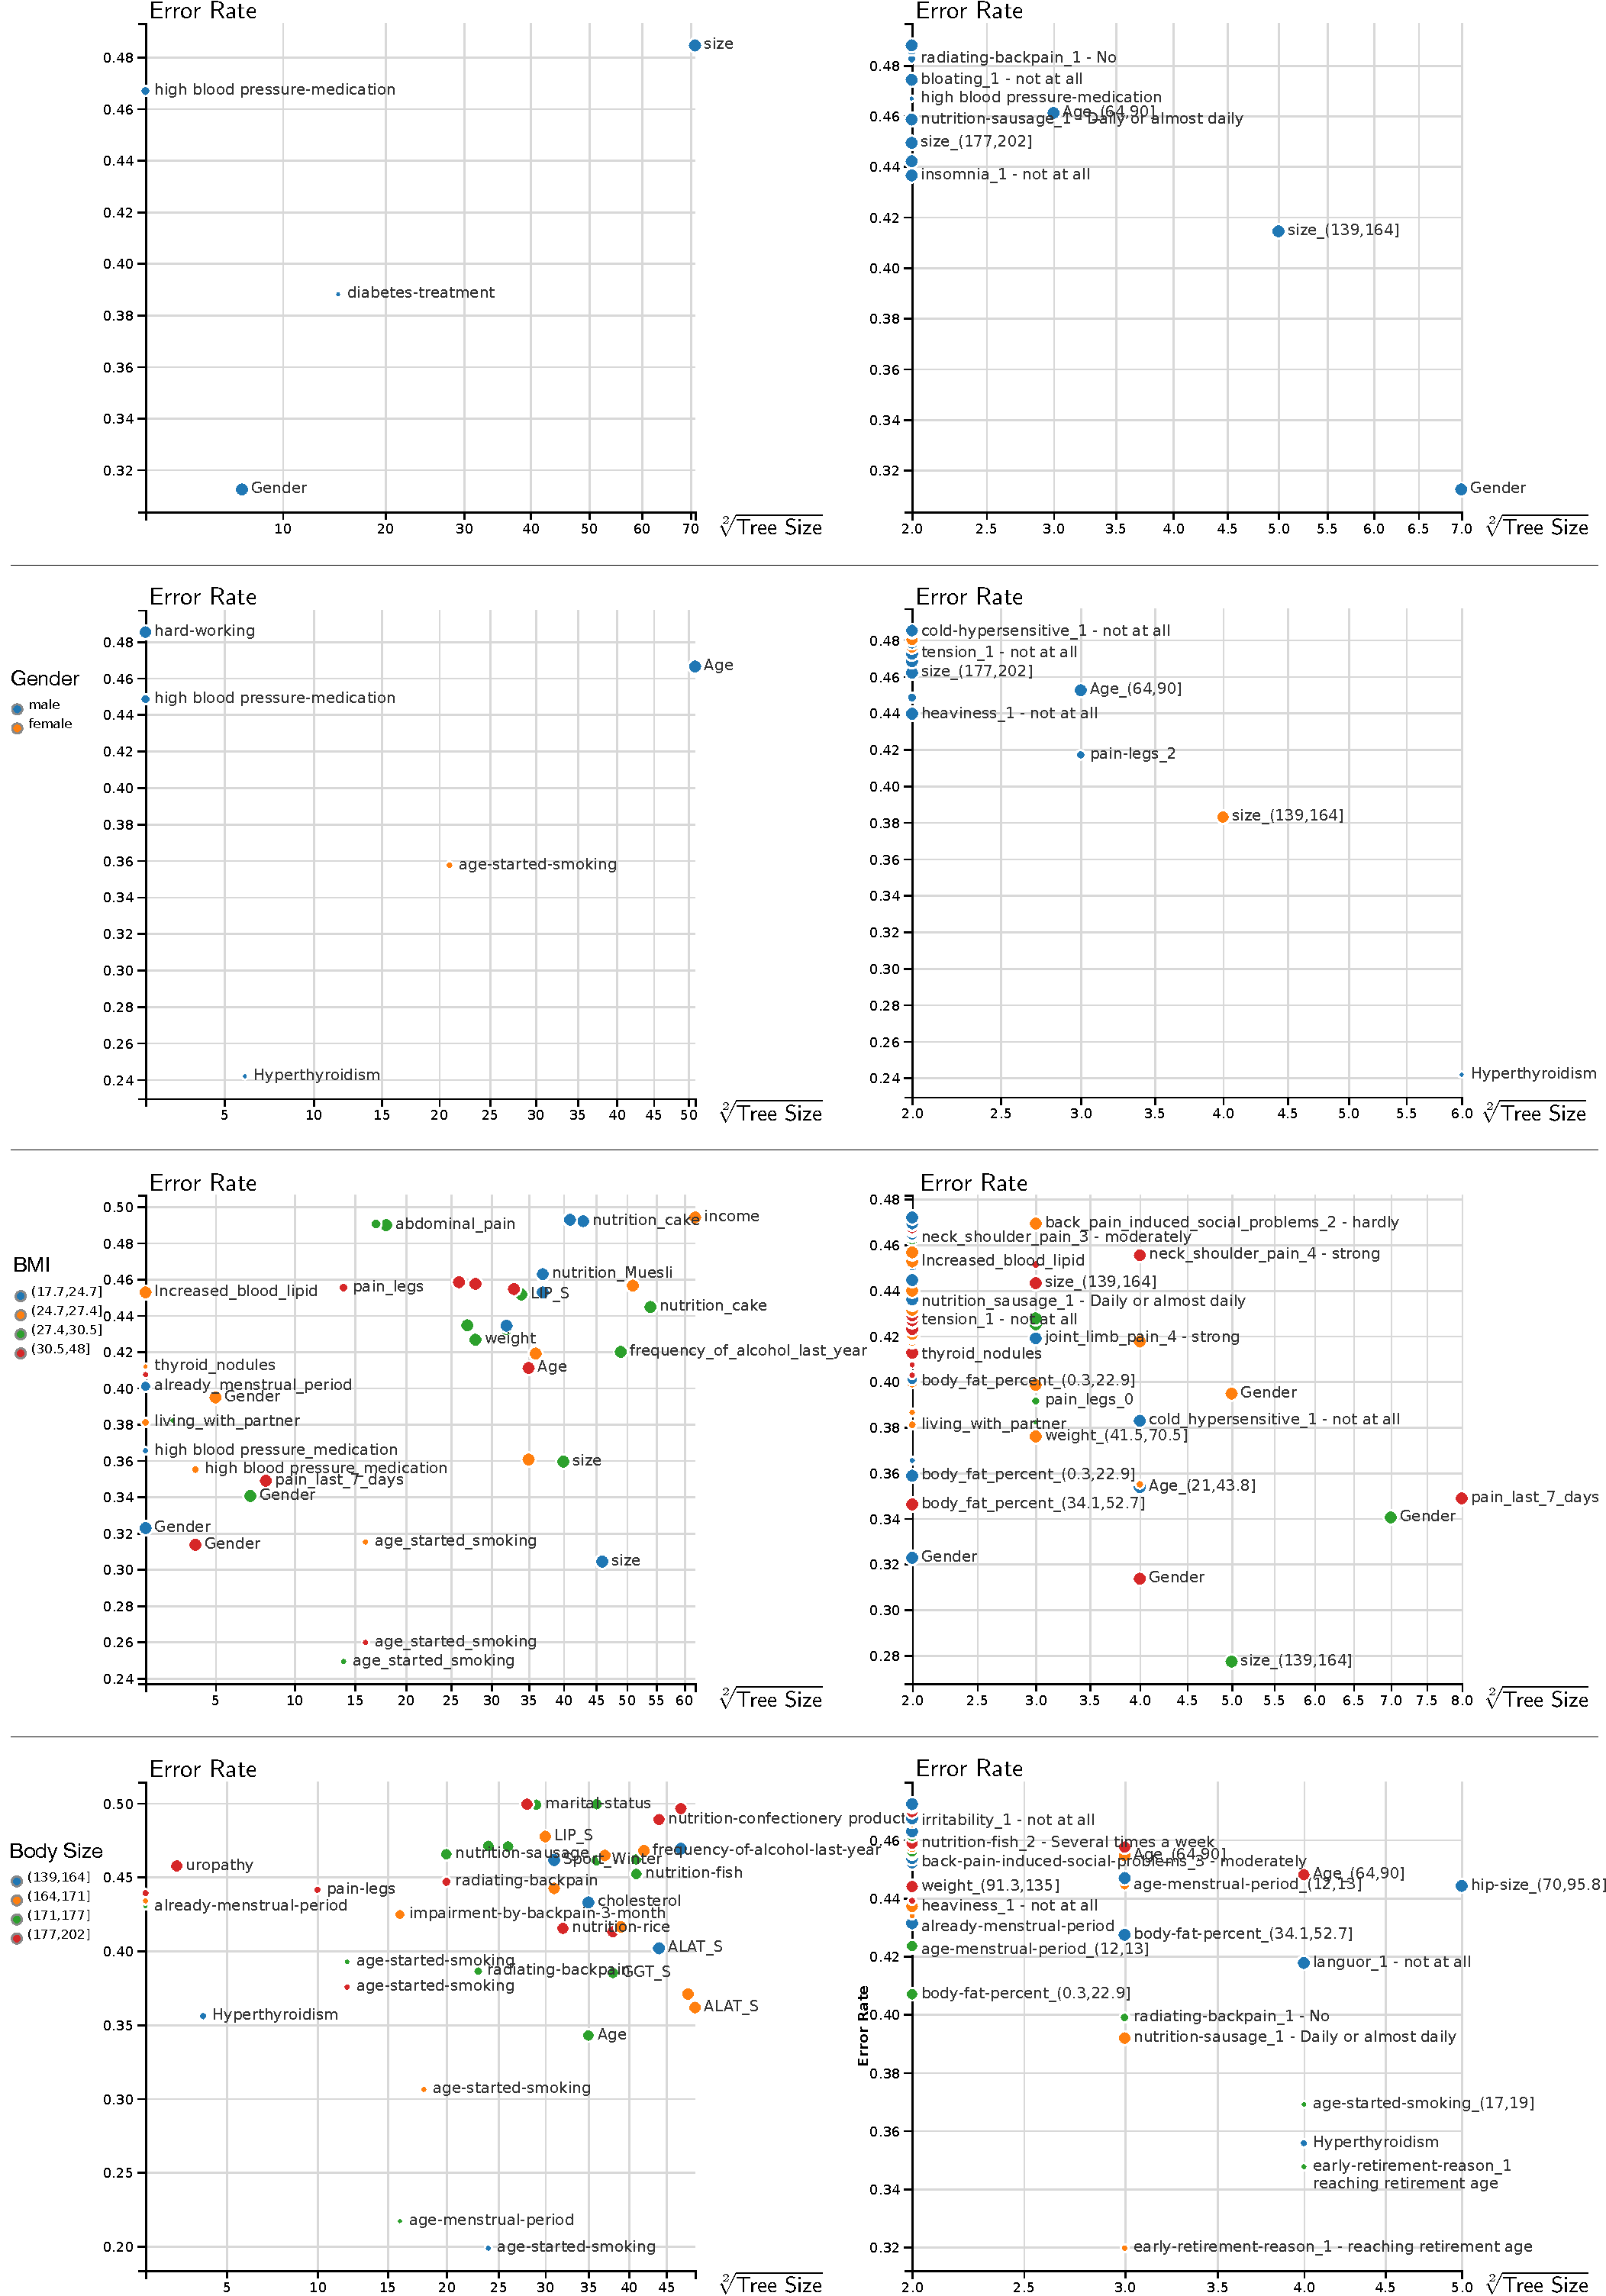
\includegraphics[width=0.95\textwidth]{figures/results}
  \caption{
%%
Interactive scatter plot visualization of all C5.0 classification results.
%%
The x-axis shows the number of decisions of the underlying model, the y-axis the classification error (see Section~\ref{subsec:VisualizationOfClassificationResults}).
%%
The left scatter plot shows the results for all variables, either metrics expressed via their quantiles, or categorical.
%%
The right scatter plot displays the dummy variables derived from the original variables.
%%
Group affiliation of a data point is color coded:
%%
no group (a), subdivision into \emph{male} and \emph{female} subjects (b), quartiles of \emph{Body Mass Index} (\emph{BMI}) (c) and quartiles of \emph{body size} (d).
%%
The number of subjects represented in a variable is denoted using the dot diameter.
%%
We only display variables with an error below $0.5$, results above this threshold are inaccurate.
%%
The interactive plot (see supplemental material) has clickable data points, displaying corresponding decision tree in a tool tip.
%%
}
  \label{fig:results}
\end{figure*}
\noindent In this section, we show which non-image variables can be explained using the 9 image derived variables.
%%
We also create subject groups to assess the influence of variables affecting the lumbar spine shape.
%%
We carry out the analysis using different subject groups:
\begin{enumerate}
	%%
	\item All subjects,
	%%
	\item subdivision into \emph{male} and \emph{female},
	%%
	\item subdivision by \emph{Body Mass Index quantiles} ($BMI = \frac{m}{l^2}$ where $m$ is the \emph{body mass} in kilogram and $l$ is the \emph{body size} in meter), yielding the groups (17, 24.7] (24.7, 27.4] (27.4, 30.5] (30.5, 48],
	%%
	\item subdivision by \emph{size quantiles}, yielding the groups (139, 164], (164, 171], (171, 177], (177, 202].
	%%
\end{enumerate}
%%
We plotted each group twice.
%%
The first plot shows all original variables.
%%
The second plot shows all categorical variables transformed into dichotomous dummy variables. % (recall subsection~\ref{sec:C5.0}).
%%
The shown mutual dependencies aim to amplify \emph{hypothesis generation}.
%%
Dedicated statistical analysis of these results solely focussed on epidemiological research is not the scope of this paper.
%%
\subsection{All Variables}
%%
The vast majority of non-image variables cannot be automatically classified based on the image-variables.
%%
This is reflected in the large amount of variables classified with an error above $0.6$.
%%

None of the pain indicators can be described reliably using the image-based variables.
%%
The only variable reliably classified in this group is \emph{gender}, which can be predicted with an error of $0.31$ using 7 rules and incorporates only \emph{curvature-} and \emph{curvature angle}-related variables.
%
%%
The distinctness lies in the average difference in \emph{body size} between \emph{male} and \emph{female} subjects.
%%
\emph{Medication for high blood pressure} is classified for 1,058 subjects with an error of $0.47$ solely based on \emph{coronal mean curvature}.
%%
Almost all subjects who are medicated ($796$ of $1,058$) were correctly classified.
%%
The vast majority of non-medicated subjects ($262$ of $1,058$) are false-positive classified, yielding a poor quality of the classifier w.r.t epidemiological research.
%%
The four \emph{body size} groups could be characterized with an error of $0.48$, but the decision tree comprises 71 rules and imposes overfitting.

The analysis of the dummy variables yields a result similar to the \emph{blood pressure medication}.
%%
Variables, such as subjects sized 139-164 cm, between 64 and 90 years of \emph{age} or \emph{nutrition}-related variables are dominantly populated by one manifestation.
%%
The classifier neglects the other group and yields an error below $0.5$.
%%
\subsection{Gender Groups}
%%
Classification using groups divided by \emph{gender} do not produce satisfying results.
%%
Only \emph{hypothyroidism} could be described for male subjects with an error of $0.24$ for 110 subjects using the \emph{mean curvature} and \emph{curvature angle}.
%%
Since there are only 30 male subjects diagnosed with \emph{hypothyroidism}, the statistical power of the result is reduced.
%%
The dummy variable analysis showed that female subjects of \emph{139-164~cm body size} could be discriminated using the \emph{mean curvature} and \emph{curvature angle}, with an error of $0.38$.
%%
\subsection{Body Mass Index Groups}
%%
\emph{Gender} could be classified for each \emph{BMI} group using \emph{mean curvature} and \emph{curvature angle}.
%%
The error varies between $0.31$ (\emph{BMI} of \emph{$30.5-48$}, 4 decision rules) to $0.39$ (\emph{BMI} of \emph{$24.7-27.4$}, 5 decision rules).
%%
The starting age of smoking could be characterized well with an error between $0.25$ and $0.32$ for all \emph{BMI} groups except for subjects with a \emph{BMI} of \emph{$30.5-48$}.
%%
The result however, is probably overfitted to the data due to tree sizes between $14$ and $16$.
%%

Some variables, such as \emph{body size}, can be described with an error of $0.3$ to $0.36$, but only using large decision trees with over 20 rules.
%%
Using mostly \emph{mean curvature} and \emph{curvature angle}, the \emph{leg pain level} can be predicted using $14$ rules with an error of $0.46$ for obese subjects (\emph{BMI} higher than $30$).
%%
The dichotomous variable whether the subject has felt \emph{pain in the last seven days} can also be predicted for this group using the same features.
%%
The resulting tree consists of $8$ rules and has an error of $0.35$.
%%
Obese subjects are prone to \emph{back} and \emph{leg pain} due to a more stressed lumbar spine.
%%
The stress-induced spine deformation seems to directly influence the pain levels for these subjects.

The dummy variable analysis shows many results using a decision tree with one rule based on \emph{mean curvature} or \emph{curvature angle} with an error between $0.35$ and $0.47$.
%%
\subsection{Size Groups}
%%
Many previously described results are influenced by \emph{subject size}.
%%
Differences between \emph{male} and \emph{female} subjects can be explained by the average \emph{body size} difference.
%%
For example, large subjects are already characterized by their rather straight spine.
%
The question is whether the inter-group spine variability parameter is sufficient for predicting other variables or not.
%%
Dividing subjects into \emph{body size} groups potentially highlights classifications not influenced by \emph{body size}.
%%
\\\\
\noindent \textbf{Large Decision Trees.}
Back pain-associated variables can be explained for various \emph{size} groups, but we could not extract universal rules.
%%
\emph{Radiating back pain} could be described with an error of $0.39$ using 23 rules for subjects between \emph{$171-177~cm$ body size} with \emph{torsion} and \emph{mean curvature}.
%%
For subjects sized \emph{$177-202~cm$} the error increases to $0.47$ using 20 decision rules.
%%
There are several decision trees for laboratory values, e.g. \emph{alanine aminotransferase} value (relevant for diagnosis of liver or gallbladder illness) in the blood can be described with an error of $0.4$ (\emph{$139-164~cm$}) to $0.36$ (\emph{$164 - 171~cm$}).
%%
Similar values can be observed for \emph{cholesterol} or \emph{age}.
%%
Due to the large decision trees, these results are not usable and impose overfitting to the data.
%%
\\\\
\noindent \textbf{Small Decision Trees.}
%%
The dummy variables show several variables described using only one decision rule with an error between $0.42$ and $0.47$.
%%
Most of these variables have a dominant manifestation and the classifier shows a low detection precision for the second manifestation.
%%
These variables include \emph{nutrition}, \emph{thyroid disorder} and \emph{social problems induced by back pain}.
%%
%TODO: [medium] Muss das rein? Auswertung der Anteile der Parameter an den Ergebnissen (Torsion, Curvature, etc. - welches ist der dominanteste Parameter?)
%%
\section{\uppercase{Conclusion}}
\label{sec:Conclusion}
\noindent The presented results indicate that the image-based variables \emph{torsion}, \emph{curvature} and \emph{curvature angle} are not sufficient to characterize pathological changes in the lumbar spine in the given quality.
%%
They are associated with subject \emph{gender} due to their \emph{body size} difference using \emph{mean curvature} and \emph{mean curvature angle}.
%%
This is due to the higher curvature of smaller subjects and the significant difference of average \emph{body size} between male and female.
%%
\emph{Gender} was detected well in the analysis of all subjects as well as subjects divided by \emph{BMI}.

Subjects grouped using \emph{body size} have a similar spine shape and a lower variance.
%%
The remaining information within these groups is not sufficient to characterize back pain-related variables.
%%
Associations with certain \emph{nutrition} or \emph{psychological} variables can be observed with a comparatively high error for some \emph{body size} groups.
%%

Another observation during the analysis is that large decision trees achieve low error scores.
%%
Their complexity imposes overfitting to the data and they are not suitable for extracting universal rules.
%%
\\\\
\noindent \textbf{Applicability.}
%%
Classification methods based on decision trees have proven to be useful for assessing the discriminative power of a variable set.
%%
Their ability to consider variable combinations makes them more powerful than correlation coefficients calculated for each variable.
%%
This advantage comes with a much more complex output, the results are more challenging to assess and to abstract.
%%
Our method to plot derived metrics and custom-tailored error measures proved to be effective.
%%
Huge result spaces could be navigated fast using our interactive visualization.
%%
Therefore, the method is applicable not only for deriving information based on image data, but on all potential target variables.
%%

% BLIND
%As described in a prior work (\cite{Klemm2014VIS}), the suggestion of potentially interesting features when analyzing a condition is an important aspect of visual analytics in epidemiology.
Suggesting potentially interesting features when analyzing a condition is an important aspect of visual analytics in epidemiology.
%%
We can achieve this also using the presented method by trying to describe several (dichotomous) target values with a decision tree constructed from all available data.
%%
This allows to assess both the discriminative power of the data set regarding the target variables, and as the most important variables for the classification.
%%
\\\\
\noindent \textbf{Predictive Power of Image-Derived Variables.}
We showed that \emph{torsion}, \emph{curvature} and \emph{curvature angle} of the lumbar spine at the presented precision are not sufficient to characterize lumbar back pain in the SHIP data set.
%%
Our method allowed to assess their discriminative power, which is largely limited for separating male and female subjects, \emph{nutrition} variables, as well as different disease indicators.
%%
The C4.5 algorithm proved to be an effective tool for evaluating a set of derived metrics regarding their suitability to classify non-image variables.
%%
Over-fitting to the data indicated by complex decision trees has to be taken into account as well.
%%
\\\\
\noindent \textbf{Future Work.}
%% Contributions
We provide a method for comparative analysis of decision trees independent of the variable manifestation count using interactive scatter plots.
%%
We applied the technique to gain insight into the predictive power of 9 image-derived variables for 134 non-image variables.
%%
The analysis was carried out for subjects divided by \emph{gender}, \emph{BMI}, and \emph{body size} to assess their influence on the lumbar spine shape.

The methods presented herein may be applied to comprehensive epidemiological data sets to learn more about mutual dependencies among variables and to generate hypotheses on potential associations and subgroups.
%
These hypotheses, however, have to be substantiated by dedicated statistical analyses and replication in independent cohorts.

In our future work, we will focus on more precise models for extracting measures.
%%
Dented vertebras are an early sign of a pathological deformation, so we want to capture this by segmenting the top and bottom point of each vertebra center.
%%
Another interesting metric is the spine canal thickness over the whole spine, capturing early signs of herniated disc disease.
%%
As another focus, we want to include the method into existing visual analytics methods designed for analyzing shape information for epidemiological data \cite{Klemm2014VIS}.
%%
\\\\
Combining the power of statistical analysis, visual analytics and data mining techniques are essential for analyzing increasingly complex heterogenous population data.
%%
These methods do not aim to replace the traditional epidemiological workflow, but rather intervene at the weak points of standard statistical methods.
%%
Our method provides a novel way to gain insight into these complex data sets and amplifies hypotheses generation.

\section*{\uppercase{Acknowledgements}}
\begin{small}
\noindent SHIP is part of the Community Medicine Research net of the University of Greifswald, Germany, which is funded by the Federal Ministry of Education and Research (grant no. 03ZIK012), the Ministry of Cultural Affairs as well as the Social Ministry of the Federal State of Mecklenburg-West Pomerania. Whole-body MR imaging was supported by a joint grant from Siemens Healthcare, Erlangen, Germany and the Federal State of Mecklenburg-Vorpommern. The University of Greifswald is a member of the ‘Centre of Knowledge Interchange’ program of the Siemens AG. This work was supported by the DFG Priority Program 1335: Scalable Visual Analytics.
\end{small}


\vfill
\bibliographystyle{style/apalike}
{\small
\bibliography{bibliography}}

%\section*{\uppercase{Appendix}}
%\noindent The IVA tool and all shown plots presented in this paper are available as supplementary material under the following link: \url{blind.dnsalias.com}.

\vfill
\end{document}